\documentclass{kdiartcl}

\usepackage{amsmath}
\usetikzlibrary{arrows.meta,decorations.pathreplacing}

\university{HTWG Konstanz}
\institute{Fachbereich Angewandte Informatik}
\lecture{Rechnernetze}
\date{\today}

\author{Paul Krüssel}
\title{Lösung Theorieaufgabe 1}
%\subtitle{Abgabeende: 14. April 2026}

\singlespacing

\begin{document}
\maketitle

\section{Ende-zu-Ende-Verzögerung}

\subsection{Bestimung der Ausbreitungsverzögerung und Übertragungsverzögerung}

Die Ausbreitungsverzögerung lässt sich mit dieser Formel berechnen:

\[
t_{prop} = \frac{l}{v}
\]

mit \( l \) als Länge des Links in $m$ und \( v \) als Ausbreitungsgeschwindigkeit in \( \frac{m}{s} \).


Die Übertragungsverzögerung lässt sich mit dieser Formel berechnen:

\[
    t_{tx} = \frac{L}{C}
\]
    
mit \( L \) als Paketgröße in Bit und \( C \) als Datenrate in Bit/s.
    
\subsubsection{Berechnung Link 1}
    Für Link 1 sind folgende Größen gegeben: \\
    \begin{itemize}
        \item $C = 60 Mbps = 60.000.000 \frac{b}{s}$
        \item $L = 1500 Byte = 12000 b$
        \item $l = 15m$
        \item $v = 300.000 \frac{km}{s} = 300.000.000 \frac{m}{s}$
    \end{itemize}
    Ausbreitungsgeschwindigkeit: \\
    \begin{center}
        $t_{prop} = \frac{L}{C} = \frac{12000 b}{60.000.000 \frac{b}{s}} = 2 * 10^{-4}s$
    \end{center}
    Übertragungsverzögerung: \\
    \begin{center}
        $t_{tx} = \frac{l}{v} = \frac{15m}{300.000.000\frac{m}{s}} = 5 * 10^{-8}s$
    \end{center}
\subsubsection{Berechnung Link 2}
    Für Link 2 sind folgende Größen gegeben: \\
    \begin{itemize}
        \item $C = 25 Mbps = 25.000.000 \frac{b}{s}$
        \item $L = 1500 Byte = 12000 b$
        \item $l = 250m$
        \item $v = 200.000 \frac{km}{s} = 200.000.000 \frac{m}{s}$
    \end{itemize}
    Ausbreitungsgeschwindigkeit: \\
    \begin{center}
        $t_{prop} = \frac{L}{C} = \frac{12000 b}{25.000.000 \frac{b}{s}} = 4.8 * 10^{-4}s$
    \end{center}
    Übertragungsverzögerung: \\
    \begin{center}
        $t_{tx} = \frac{l}{v} = \frac{250m}{200.000.000\frac{m}{s}} = 1.25 * 10^{-6}s$
    \end{center}
\subsubsection{Berechnung Link 3}
    Für Link 3 sind folgende Größen gegeben: \\
    \begin{itemize}
        \item $C = 20 Gbps = 20.000.000.000 \frac{b}{s}$
        \item $L = 1500 Byte = 12000 b$
        \item $l = 10km = 10.000m$
        \item $v = 250.000 \frac{km}{s} = 250.000.000 \frac{m}{s}$
    \end{itemize}
    Ausbreitungsgeschwindigkeit: \\
    \begin{center}
        $t_{prop} = \frac{L}{C} = \frac{12000 b}{20.000.000.000 \frac{b}{s}} = 6 * 10^{-7}s$
    \end{center}
    Übertragungsverzögerung: \\
    \begin{center}
        $t_{tx} = \frac{l}{v} = \frac{10.000m}{250.000.000\frac{m}{s}} = 4 * 10^{-5}s$
    \end{center}

\subsection{Ende-zu-Ende-Verzögerung}
    Die Ende-zu-Ende-Verzögerung lässt sich mit dieser Formel berechnen: \\
    \begin{center}
        $d_{e2e} = \sum t_{tx,i} + \sum t_{prop,i}$ $ mit$ $i$ $als$ $Linknummer$ \\
    \end{center}
    Anhand dieser Formel kann man erkennen, dass die Reihenfolge egal ist. \\
    Einsetzen der Werte in die Formel: \\
    \begin{center}
        $\sum t_{tx,i} = 2 * 10^{-4}s + 4.8 * 10^{-4} + 6 * 10^{-7}s = 6.8006 * 10^{-4}s$ \\
        $\sum t_{prop,i} = 5 * 10^{-8}s + 1.25 * 10^{-6}s + 4 * 10 ^ {-5} = 4.013 * 10^{-5}s$ \\
        $d_{e2e} = 6.8006 * 10^{-4}s + 4.013 * 10^{-5}s = 7.2019 * 10^{-4}s$
    \end{center}

\subsection{Packet-Burst}
    Die Reihenfolge macht auch hier wieder keinen Unterschied, da die Formel für die Gesamtdauer eines Packet-Burst mit $n$ Paketen lediglich aufsummiert: \\
    \begin{center}
        $T_{E2E}(n) = T_{E2E}(1) + (n-1) * max(t_{tx,i})$
    \end{center}
    Einsetzen in die Formel: \\
    \begin{center}
        $T_{E2E}(20) = 7.2019 * 10^{-4}s + 19 * (4.8 * 10^-{4}s) = 9.84019ms$
    \end{center}

\section{Durchsatz und Paketverlust (Standard-Klausuraufgabe)}
    \subsection{Bestimmung Ende-zu-Ende für ein Paket}
    Berechnung der gesamten Ausbreitungsverzögerung: \\
    \begin{center}
        $t_{prop} = \sum t_{prop, R_i} = 4ms + 72ms + 72ms + 5ms + 5ms = 158ms$ \\
    \end{center}
    Berechnung der gesamten Übertragungsverzögerung: \\
    \begin{center}
        $t_{tx} = \sum t_{tx, R_i} = 4ms + (1,20 / 0,2) * 4ms + (1,20 / 0,3) * 4ms + (1,20 / 0,15) * 4ms + (1,20 / 0,05) * 4ms = 4ms + 24ms + 16ms + 32ms + 96ms = 172ms$
    \end{center}
    Berechnung der Ende-zu-Ende Übertragungsdauer für ein Paket: \\
    \begin{center}
        $T_{E2E} = t_{prop} + t_{tx} = 158ms + 172ms = 330ms$
    \end{center}

    \subsection{Paketverlust}
    Die Quelle versendet ein Paket alle $8ms$, also beträgt die Paketrate $\frac{1}{8ms} = 125 Pakete/s$
    \subsubsection*{(a)}
    Die maximalen Bedienrate läst sich so berechnen: \\
    $Q \rightarrow Z = \frac{1}{t_{tx}}$\\
    Die maximalen Bedienraten der Links sind: \\
    \begin{center}
        $\mu_{Q \rightarrow R_1} = \frac{1}{4ms} = 250$ $Pakete/s$ \\
        $\mu_{R_1 \rightarrow R_2} = \frac{1}{24ms} \approx 41,67$ $Pakete/s$ \\
        $\mu_{R_2 \rightarrow R_3} = \frac{1}{16ms} = 62,5$ $Pakete/s$ \\
        $\mu_{R_3 \rightarrow R_4} = \frac{1}{32ms} = 31,25$ $Pakete/s$ \\
        $\mu_{R_4 \rightarrow Z} = \frac{1}{96ms} \approx 10,42$ $Pakete/s$
    \end{center}
    Wenn langfristig mehr Pakete ankommen, als ein Link weiterleiten kann, dann wird der überschüssige Anteil verworfen. Dieser Verlustanteil lässt sich so berechnen: \\
    \begin{center}
        $p_{Verlust} = 1 - \frac{\mu}{\lambda{in}} (\lambda_{in} > \mu)$
    \end{center}
    \begin{tabular}{c c c c}
        \hline
        Link & ankommende Rate ($Pakete/s$) & Bedienrate ($Pakete/s$) & Verlustanteil \\
        \hline
        $Q \rightarrow R_1$ & 125,00 & 250,00 & 0\% \\
        $R_1 \rightarrow R_2$ & 125,00 & 41,67 & $1 - \frac{41,67}{125} = 66,67\%$ \\
        $R_2 \rightarrow R_3$ & 41,67 & 62,50 & 0\% \\
        $R_3 \rightarrow R_4$ & 41,67 & 31,25 & $1 - \frac{41,67}{31,25} = 25,00\%$ \\
        $R_4 \rightarrow Z $ & 31,25 & 10,42 & $1 - \frac{31,25}{10,42} = 66,67\%$ \\
        \hline
    \end{tabular}
    \pagebreak
    \subsubsection*{(b)}
    Gegeben ist die Ausbreitungsgeschwindigkeit mit $v = 200.000 \frac{km}{s} = 2 * 10^{8}\frac{m}{s}$ \\
    Die Ausbreitungsverzögerung für den Link $R_1 \rightarrow R_2$ beträgt $72ms$. Damit ist die physikalische Länge des Links: \\
    \begin{center}
        $l = v * t_{prop} = 2 * 10^8 \frac{m}{s} * 0,024s = 1,44 * 10^7 = 14.400km$
    \end{center}
    Die physikalische Länge eines Pakets auf diesem Link ergibt sich aus der Übertragungszeit von $24ms$:\\
    \begin{center}
        $l_{Paket} = v * t_{tx} = 2*10^8 \frac{m}{s} * 0,024s = 4,8 * 10^6m = 4800km$
    \end{center}
    Anzahl gleichzeitig sich auf dem Link befindender Pakete: \\
    \begin{center}
        $N_{Pakete} = \frac{l}{l_{Paket}} = \frac{14400}{4800} = 3$
    \end{center}

    \subsection{Skizzierung der physikalischen Ausdehnung}
    Der Link $R_1 \rightarrow R_2$ ist der erste Flaschenhals, weshalb die Pakete ohne Abstand die gesamte Leitung ausnutzen. Oben habe ich bereits die physikalische Länge eines Pakets für diesen Link berechnet. \\
    Der Link $R_2 \rightarrow R_3$ ist kein Flaschenhals, weshalb es einen Abstand zwischen diesen Paketen gibt. \\
    Da dieser Link genauso wie der erste Link eine Ausbreitungsverzögerung von $72ms$ hat und dieselbe Ausbreitungsgeschwindigkeit von $200.000km/s$ hat, ist dieser Link ergibt sich die gleiche Länge: \\
    \begin{center}
        $l = 14.400km$
    \end{center}

    Die Übertragungsverzögerung ist hier $16ms$. Also ist die physikalische Länge eines Pakets: \\
    \begin{center}
        $l_{Paket} = 2 * 10^{8} \frac{m}{s} + 0,016s = 3,2 * 10^6m = 3200km$
    \end{center}
    Da aus $R_1 \rightarrow R_2$ alle $24ms$ ein Paket ankommt, dieses allerdings bereits innerhalb von $16ms$ übertragen wird, ergibt sich eine Übertragungslücke von \\ 
    \begin{center}
        $24ms - 16ms = 8ms$
    \end{center}

    Die physikalische Länge der Leerlücke beträgt: \\
    \begin{center}
        $l_{Lücke} = 2 * 10^8\frac{m}{s} * 0.008s = 1,6 * 10^6m = 1600km$
    \end{center}

    Daraus ergibt sich diese Skizze:
    

    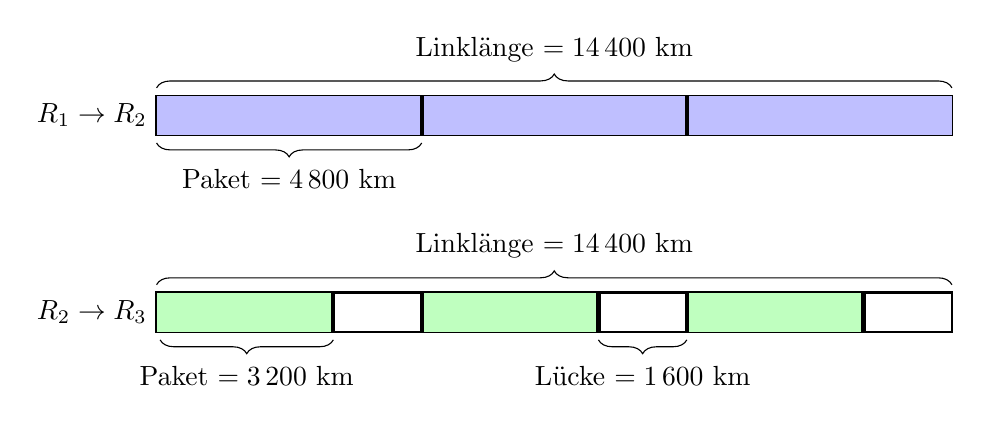
\begin{tikzpicture}[x=0.0007cm,y=0.5cm,>=Latex]
        % =========================================================
        % SKALIERUNG:
        % 14400 km = gesamte Balkenlaenge
        % =========================================================

        % ---------------------------------------------------------
        % Erster Link: R1 -> R2
        % Linklaenge: 14400 km
        % Paketlaenge: 4800 km
        % Abstand: 0 km
        % ---------------------------------------------------------

        \node[left] at (0,5.5) {$R_1 \rightarrow R_2$};

        % Aussenrahmen des Links
        \draw[thick] (0,5) rectangle (14400,6);

        % Pakete
        \fill[blue!25] (0,5) rectangle (4800,6);
        \fill[blue!25] (4800,5) rectangle (9600,6);
        \fill[blue!25] (9600,5) rectangle (14400,6);

        % Dicke Trennlinien zwischen den Paketen
        \draw[line width=1.5pt] (4800,5) -- (4800,6);
        \draw[line width=1.5pt] (9600,5) -- (9600,6);

        % Beschriftung Linklaenge
        \draw[decorate,decoration={brace,amplitude=5pt}]
        (0,6.2) -- (14400,6.2)
        node[midway,above=6pt] {Linklänge $= 14\,400\ \mathrm{km}$};

        % Beschriftung Paketlaenge
        \draw[decorate,decoration={brace,mirror,amplitude=5pt}]
        (0,4.8) -- (4800,4.8)
        node[midway,below=6pt] {Paket $= 4\,800\ \mathrm{km}$};

        % ---------------------------------------------------------
        % Zweiter Link: R2 -> R3
        % Linklaenge: 14400 km
        % Paketlaenge: 3200 km
        % Luecke: 1600 km
        % ---------------------------------------------------------


        \node[left] at (0,0.5) {$R_2 \rightarrow R_3$};

        \draw[thick] (0,0) rectangle (14400,1);

        % Pakete + Lücken
        \fill[green!25] (0,0) rectangle (3200,1);
        \fill[green!25] (4800,0) rectangle (8000,1);
        \fill[green!25] (9600,0) rectangle (12800,1);

        % Trennlinien
        \draw[line width=1.5pt] (3200,0) -- (3200,1);
        \draw[line width=1.5pt] (4800,0) -- (4800,1);
        \draw[line width=1.5pt] (8000,0) -- (8000,1);
        \draw[line width=1.5pt] (9600,0) -- (9600,1);
        \draw[line width=1.5pt] (12800,0) -- (12800,1);

        % Beschriftungen
        \draw[decorate,decoration={brace,amplitude=5pt}]
        (0,1.2) -- (14400,1.2)
        node[midway,above=6pt] {Linklänge $= 14\,400\ \mathrm{km}$};

        \draw[decorate,decoration={brace,mirror,amplitude=5pt}]
        (064,-0.2) -- (3200,-0.2)
        node[midway,below=6pt] {Paket $= 3\,200\ \mathrm{km}$};

        \draw[decorate,decoration={brace,mirror,amplitude=5pt}]
        (8000,-0.2) -- (9600,-0.2)
        node[midway,below=6pt] {Lücke $= 1\,600\ \mathrm{km}$};
        
    \end{tikzpicture}

    \subsection{Ereignistabelle für den Ausgangspuffer}
    Diese Pakete werden erzeugt:
    \begin{center}
        \begin{tabular}{c c c}
            \hline
            Paket & Erzeugungszeit[ms] & Größe[B] \\
            \hline
            $P_1$ & $0,0$ & $900,0$ \\
            $P_2$ & $2,0$ & $600,0$ \\
            $P_3$ & $3,0$ & $900,0$ \\
            $P_4$ & $4,0$ & $900,0$ \\
            $P_5$ & $5,0$ & $900,0$ \\
            $P_6$ & $7,0$ & $1200,0$ \\
            $P_7$ & $9,0$ & $900,0$ \\
            $P_8$ & $24,0$ & $1200,0$ \\
            $P_9$ & $26,0$ & $1200,0$ \\
            $P_{10}$ & $27,0$ & $1200,0$ \\
            \hline
        \end{tabular}
    \end{center}

    Auf dem Link $Q \rightarrow R_1$ ergibt sich mit $1,2 Mbps$ diese Übertragungszeiten: \\
    \begin{center}
        $900 B = \frac{7200b}{1,2 * 10^6} = 0.006s = 6ms$ \\
        $600 B = \frac{4800b}{1,2 * 10^6} = 0.004s = 4ms$ \\
        $1200B = \frac{9600b}{1,2 * 10^6} = 0.008s = 8ms$
    \end{center}

    Der Ausgangs-Puffer kann bis zu 3 Pakete aufnahmen. \\
    Ereignistabelle: \\
    \begin{tabular}{c c l c c}
        \hline
        Zeit [ms] & Ereignis & Pufferbelegung danach & Bemerkung \\
        \hline
        0 & $P_1$ kommt an & [] Länge: 0 & $P_1$ startet sofort, Sendezeit $0ms \rightarrow 6ms$ \\
        2 & $P_2$ kommt an & [$P_2$] Länge: 1 & wartet im Puffer \\
        3 & $P_3$ kommt an & [$P_2$, $P_3$] Länge: 2 & wartet im Puffer \\
        4 & $P_4$ kommt an & [$P_2$, $P_3$, $P_4$] Länge: 3 & wartet im Puffer \\
        5 & $P_5$ kommt an & [$P_2$, $P_3$, $P_4$] Länge: 3 & $P_5$ geht verloren, da Puffer voll \\
        6 & $P_1$ fertig & [$P_3$, $P_4$] Länge: 2 & $P_2$ startet, Sendezeit $6ms \rightarrow 10ms$ \\
        7 & $P_6$ kommt an & [$P_3$, $P_4$, $P_6$] Länge: 3 & wartet im Puffer \\
        9 & $P_7$ kommt an & [$P_3$, $P_4$, $P_6$] Länge: 3 & $P_7$ geht verloren, da Puffer voll \\
        10 & $P_2$ fertig & [$P_4$, $P_6$] Länge: 2 & $P_3$ startet, Sendezeit $10ms \rightarrow 16ms$ \\
        16 & $P_3$ fertig & [$P_6$] Länge: 1 & $P_4$ startet, Sendezeit $16ms \rightarrow 22ms$ \\
        22 & $P_4$ fertig & [] Länge: 0 & $P_6$ startet, Sendezeit $22ms \rightarrow 30ms$ \\
        24 & $P_8$ kommt an & [$P_8$] Länge: 1 & wartet im Puffer \\
        26 & $P_9$ kommt an & [$P_8$, $P_9$] Länge: 2 & wartet im Puffer \\
        27 & $P_{10}$ kommt an & [$P_8$, $P_9$, $P_{10}$] Länge: 3 & wartet im Puffer \\
        30 & $P_6$ fertig & [$P_9$, $P_{10}$] Länge: 2 & $P_8$ startet, Sendezeit $30ms \rightarrow 38ms$ \\
        38 & $P_8$ fertig & [$P_{10}$] Länge: 1 & $P_9$ startet, Sendezeit $38ms \rightarrow 46ms$ \\
        46 & $P_9$ fertig & [] Länge: 0 & $P_{10}$ startet, Sendezeit $46ms \rightarrow 54ms$ \\
        54 & $P_{10}$ fertig & [] Länge: 0 & Ende \\
        \hline \\
    \end{tabular}
    Zwischen Quelle $Q$ und Router $R_1$ gehen die Pakete $P_5$ und $P_7$ verloren.

\end{document}

